
\documentclass[oneside, 12pt]{article}
\usepackage{CJKutf8}
\usepackage{graphicx}
\usepackage[left=3.18cm, right=3.18cm, top=2.54cm, bottom=2.54cm]{geometry}
\begin{document}
\begin{CJK*}{UTF8}{bkai}

\title{計網概HW1}
\author{107061218 謝霖泳}
\date{}
\maketitle

Define the geodesic (short path) distance between two nodes as the minimum number of hops from one node to the other. Define the diameter of a network as the maximum geodesic distance among all the pairs of two nodes. Define the degree of a node as the number of links connected to that node.\\\\
1. If the diameter of a network with 100 nodes is 1, what is the minimum number of links in this network?\\
2. If the diameter of a network with 100 nodes is 2, what is the minimum number of links in this network?\\
3. For a network of 100 nodes, if the degree of every node is at most 2, what is the minimum diameter of that network?\\
4. For a network of 100 nodes, if the degree of every node is at most 3, is it possible that the diameter of this network is not greater than 5?\\

\textbf{Solution}
\begin{enumerate}
\item
diameter = 1代表每兩個node之間都有彼此連通,所以minimum number of link = $100 \choose 2$ = 4950。

\item
diameter = 2又要達到最少的link,方法是中間擺一個node,分別向外連接剩下的99個node,如下圖。故minimum number of link = 100 - 1 = 99。

\begin{center}
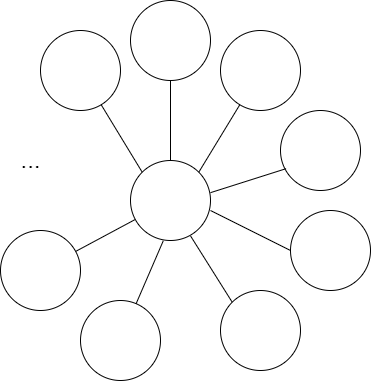
\includegraphics[width=2in]{problem2}
\end{center}

\newpage

\item
如下圖,當所有node繞成一個cycle時,diameter最小。此時的diameter = $100 / 2 = 50$。
\begin{center}
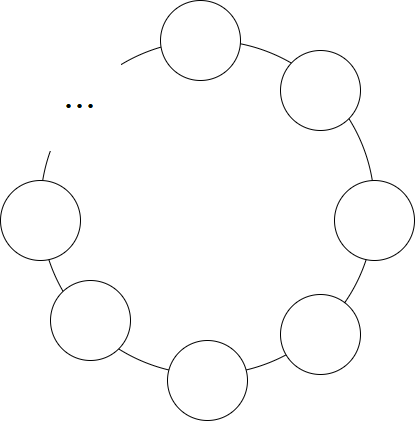
\includegraphics[width=2in]{problem3}
\end{center}

\item
考慮一個Moore Graph如下圖,要達到diameter$<=$5,maximum number of nodes $= 1 + 3*\sum_{i=0}^{4}(3-1)^i = 1 + 3 * 2 ^ 0 + 3 * 2 ^ 1 + 3 * 2 ^ 2 + 3 * 2 ^ 3 + 3 * 2 ^ 4 = 94$,而$100>94$,所以diameter不可能$<=5$,一定會多用到一層(紅色部分)。
\begin{center}
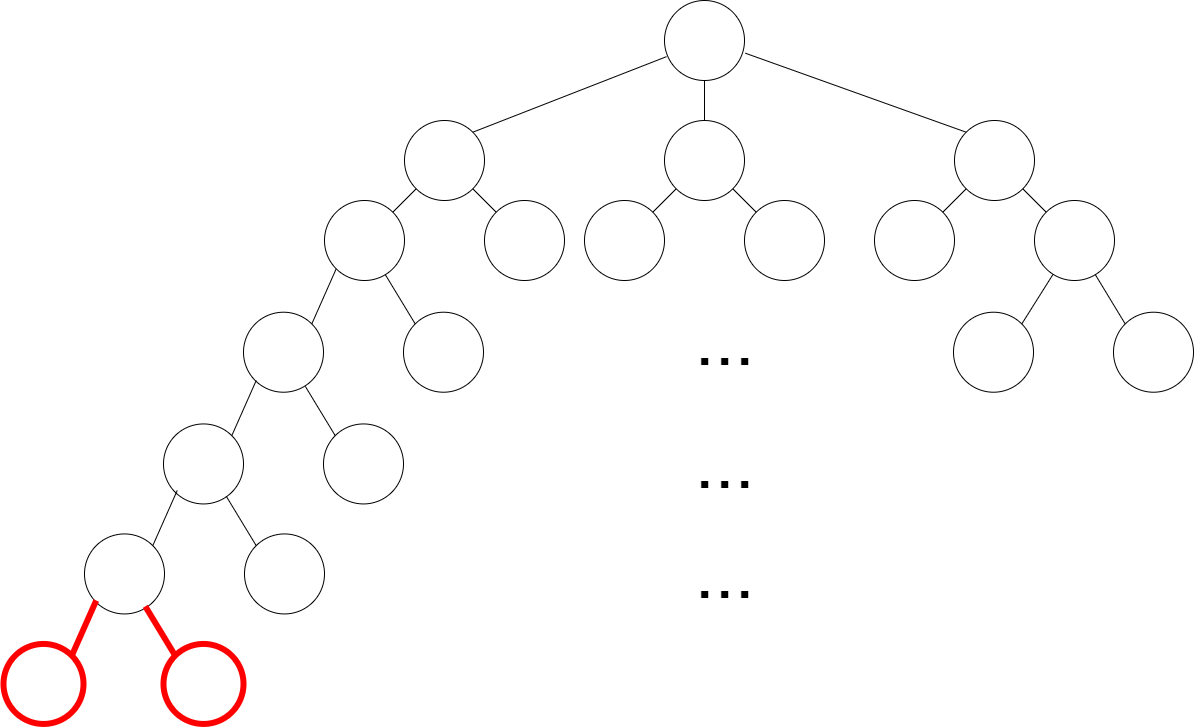
\includegraphics[width=5in]{problem4}
\end{center}

\end{enumerate}


\end{CJK*}
\end{document}